\subsection{Slave Aktuator Implementering}
\label{ch:slave_aktuator_impl}

Figur \ref{fig:topdesign_aktuator} viser topdesignet fra PSoC Creator. 

Der er porte, som styrer hhv. varmelegeme, vanding, vindue og ventilation.

Porten til ventilation styres vha. en PWM komponent. 
Det er egentlig ikke nødvendigt, men derved er blokken forberedt til PWM styring af ventilatorerne, ved senere implementering af dette; fx i forbindelse med PID regulering af temperaturen. 
Dette udnyttes samtidigt til at køre med en dutycycle på 50\%, når ventilatorerne er tændt, for at undgå for voldsom ventilation. 
Ventilatorerne startes altid med en dutycycle på 100\% i et kort øjeblik, før der skrues ned til de 50\%.
Det sker for at sikre at ventilatorerne opnår tilstrækkeligt højt omdrejningsmoment til at sætte i gang.

Det er umiddelbart oplagt at styringen af varmelegemet også foretages vha. PWM, men det er ikke muligt, da varmelegemet tændes og slukkes med et mekanisk relæ, der ikke kan håndtere høje frekvenser. 

\begin{figure}[h]
\centering 
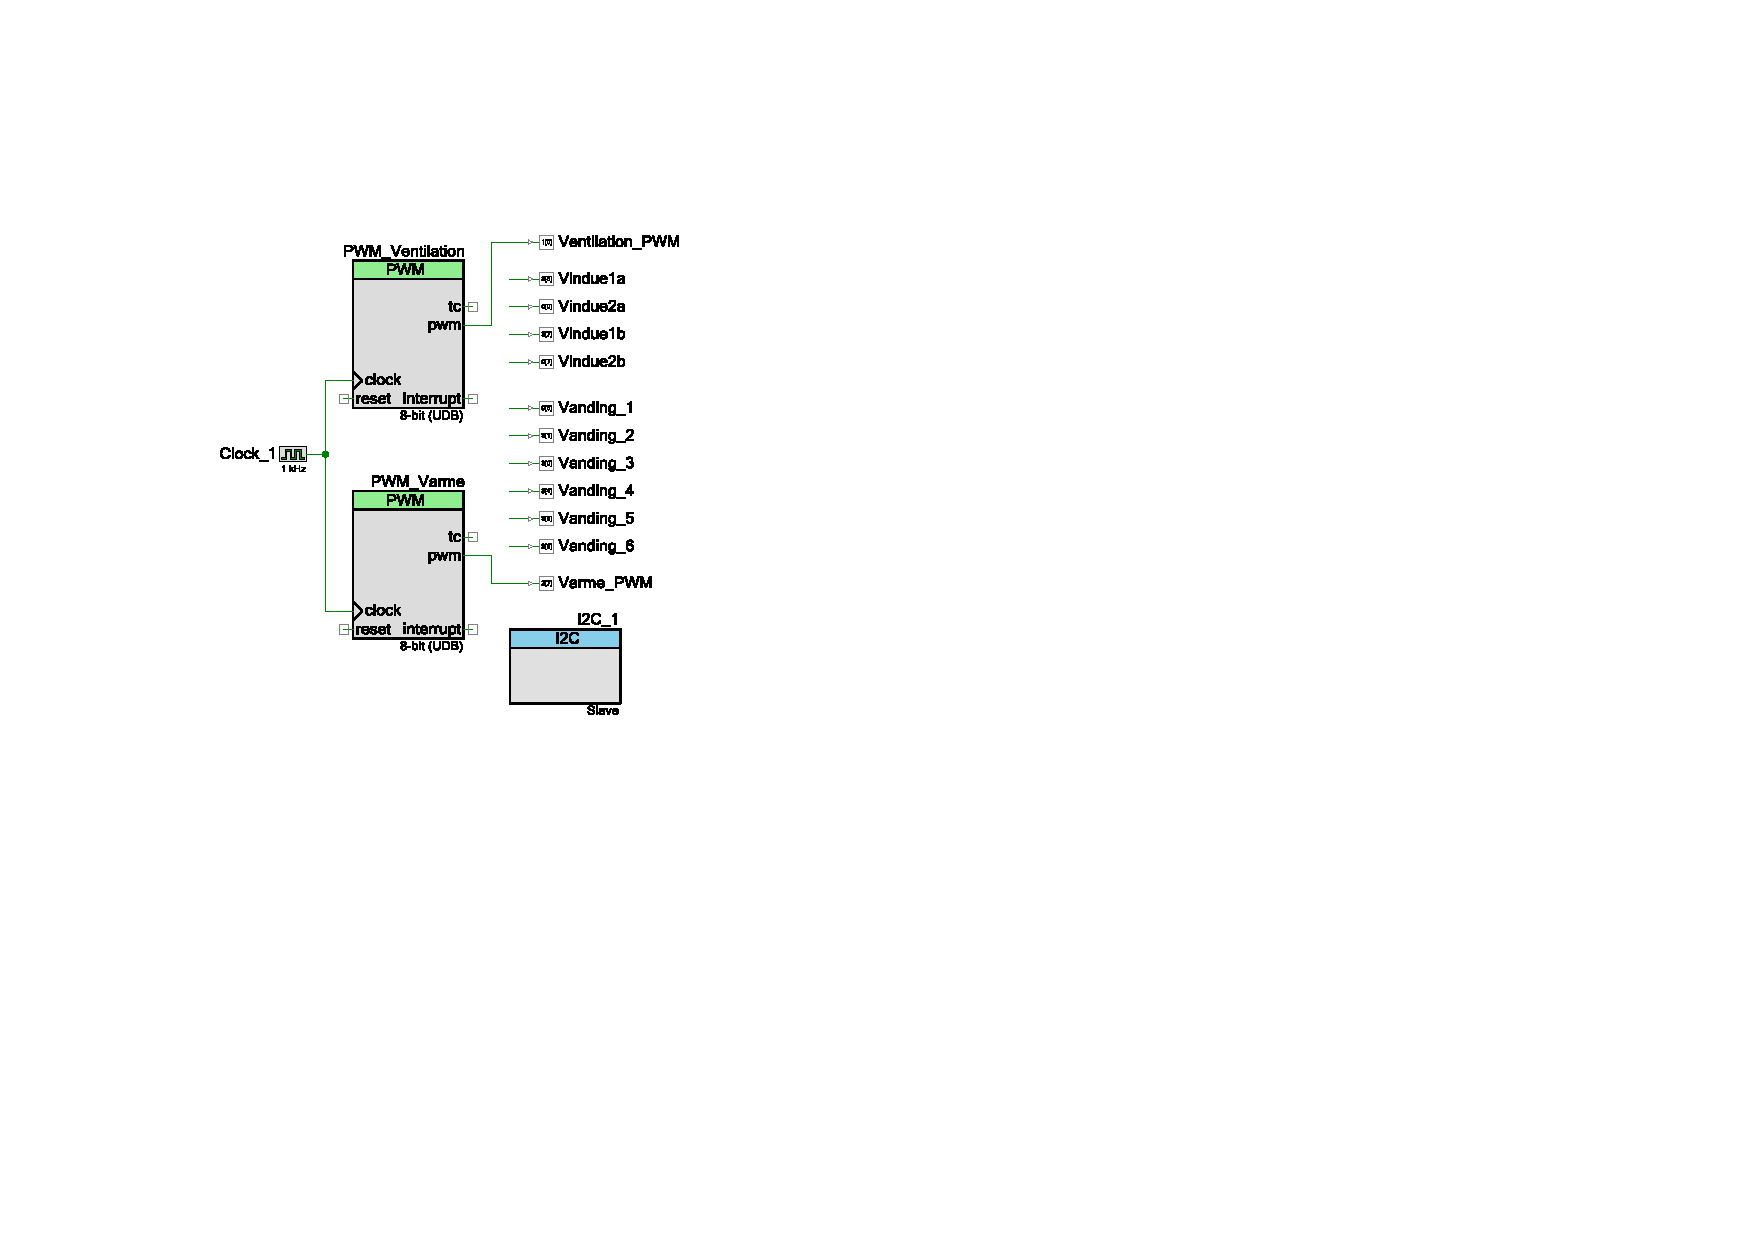
\includegraphics[width={\textwidth-8cm}, trim = 110 320 450 100, clip=true] {../fig/TopDesign_Aktuator.pdf}
\caption{TopDesign.cysch for PSoC 4 i Aktuator}
\label{fig:topdesign_aktuator}
\end{figure}

For detaljeret beskrivelse af afvikling af koden, der er anskueliggjort i state machinen under design i denne rapport (\ref{ch:slave_aktuator_design} \nameref{ch:slave_aktuator_design} Figur \ref{fig:stm_psoc_aktuator}, side \pageref{fig:stm_psoc_aktuator}), se afsnit \ref{P-subsec:sw_aktuator} \nameref{P-subsec:sw_aktuator} på side \pageref{P-subsec:sw_aktuator} i projektdokumentationen.

Print til de tre mosfet drivere til hhv. varme, ventilation og stepper motor, udlægges i Ultiboard og komponenter loddes på. 
Se fx afsnit \ref{P-subsec:vinduesmotor_impl} \nameref{P-subsec:vinduesmotor_impl} på side \pageref{P-subsec:vinduesmotor_impl} i projektdokumentationen for nærmere info derom.

\clearpage